\documentclass[conference]{IEEEtran}
\IEEEoverridecommandlockouts
\usepackage{cite}
\usepackage{amsmath,amssymb,amsfonts}
\usepackage{graphicx}
\usepackage{textcomp}
\usepackage{xcolor}
\usepackage{booktabs}
\usepackage{multirow}
\usepackage{url}
\usepackage{hyperref}

\def\BibTeX{{\rm B\kern-.05em{\sc i\kern-.025em b}\kern-.08em
    T\kern-.1667em\lower.7ex\hbox{E}\kern-.125emX}}

\begin{document}

\title{A Multi-Stage Framework for Detecting Factual Hallucinations in Large Language Model Outputs\\
{\footnotesize \textsuperscript{}}
\thanks{}
}

\author{\IEEEauthorblockN{Punya Acharya}
\IEEEauthorblockA{\textit{Department of Computer Science and Engineering} \\
\textit{Undergraduate Research Project}\\
Email: punyaa18@example.edu}
}

\maketitle

\begin{abstract}
Large Language Models (LLMs) have demonstrated remarkable capabilities in generating human-like text across diverse domains. However, these models frequently produce hallucinations—outputs containing factually incorrect or unverifiable information presented with high confidence. This phenomenon poses significant challenges for deploying LLMs in critical applications requiring factual accuracy. We present a comprehensive, multi-stage framework for detecting and quantifying hallucinations in LLM-generated text. Our approach combines claim extraction using natural language processing techniques, evidence retrieval from trusted knowledge sources, natural language inference for verification, and risk-based scoring mechanisms. The system employs transformer-based models for both claim verification and semantic similarity assessment. Through systematic evaluation on benchmark datasets containing both factually accurate and hallucinated content, our framework achieves 87.3\% accuracy in identifying contradicted claims and 82.1\% overall hallucination detection accuracy. The modular architecture supports both local deployment and integration with external LLM services, enabling flexible adaptation across different use cases. Our findings demonstrate that structured verification pipelines can effectively mitigate hallucination risks in LLM applications.
\end{abstract}

\begin{IEEEkeywords}
Large Language Models, Hallucination Detection, Natural Language Inference, Fact Verification, Claim Extraction, Knowledge Grounding
\end{IEEEkeywords}

\section{Introduction}

The rapid advancement of Large Language Models has revolutionized natural language processing applications, enabling unprecedented capabilities in text generation, question answering, and conversational systems \cite{survey_hallucination}. Models such as GPT-4, LLaMA, and Claude have demonstrated human-level performance on numerous benchmarks. Despite these achievements, a critical limitation persists: LLMs frequently generate content that appears fluent and confident but contains factual inaccuracies or fabricated information—a phenomenon termed ``hallucination'' \cite{why_hallucinate}.

Hallucinations manifest in various forms, ranging from subtle factual errors to entirely fabricated entities, dates, or relationships. Recent studies indicate that even state-of-the-art models exhibit substantial hallucination rates on knowledge-intensive tasks \cite{semantic_entropy}. The issue becomes particularly problematic in high-stakes domains such as healthcare, legal analysis, and scientific research, where factual accuracy is paramount.

The root causes of hallucinations are multifaceted. Models trained on vast internet corpora inevitably learn from incorrect or biased information. The autoregressive generation process prioritizes linguistic plausibility over factual consistency. Furthermore, LLMs lack genuine understanding of truth values and cannot reliably distinguish between memorized facts and plausible-sounding fabrications \cite{survey_hallucination}.

Existing approaches to hallucination mitigation include retrieval-augmented generation (RAG), which grounds outputs in retrieved documents, and self-consistency checking, where models evaluate their own outputs. However, these methods often require significant computational resources or architectural modifications. There remains a need for lightweight, post-hoc verification systems that can assess the factual reliability of arbitrary LLM outputs.

This paper presents a comprehensive framework for detecting hallucinations in LLM-generated text through a structured, four-stage pipeline. Our contributions include:

\begin{itemize}
\item A modular architecture combining linguistic analysis, knowledge retrieval, and inference-based verification
\item Novel claim extraction methodology leveraging entity recognition and syntactic patterns
\item Integration of multiple evidence sources with semantic relevance scoring
\item Risk-stratified scoring system enabling nuanced hallucination assessment
\item Extensive evaluation demonstrating effectiveness across diverse content types
\end{itemize}

The remainder of this paper is organized as follows: Section II reviews related work in hallucination detection and fact verification. Section III details our methodology and system architecture. Section IV describes implementation specifics. Section V presents experimental results and analysis. Section VI discusses findings and limitations, and Section VII concludes with future directions.

\section{Related Work}

\subsection{Hallucination in Large Language Models}

Recent research has extensively documented the prevalence and patterns of hallucinations in LLMs. Huang et al. \cite{survey_hallucination} provide a comprehensive taxonomy, categorizing hallucinations into factual inconsistencies, logical contradictions, and ungrounded statements. Their analysis reveals that hallucination frequency correlates with factors including prompt specificity, domain complexity, and model scale. A recent survey-style study by Cleti and Jano \cite{llmhallucination_types} further consolidates practical mitigation approaches used in production-oriented LLM systems.

The mechanisms underlying hallucinations have been studied from multiple perspectives. Farquhar et al. \cite{semantic_entropy} show that uncertainty-aware signals, such as semantic entropy, can detect many hallucination cases without altering model weights. Complementary analysis by Kalai et al. \cite{why_hallucinate} argues that hallucinations arise from incentive structures in training and evaluation that reward guessing over calibrated abstention.

\subsection{Fact Verification Systems}

Automated fact verification has evolved significantly, particularly driven by challenges like FEVER (Fact Extraction and VERification) \cite{fever_dataset}. Traditional approaches typically involve three stages: document retrieval, sentence selection, and claim classification. Recent systems employ dense retrievers with transformer-based classifiers, achieving strong performance on structured claims.

However, existing fact-checking systems often assume well-formed, explicit claims and access to curated knowledge bases. In contrast, hallucinations in LLM outputs may be subtle, implicit, or contextually embedded, requiring different detection strategies.

\subsection{Natural Language Inference}

Natural Language Inference (NLI) models, trained on datasets like SNLI and MultiNLI, classify relationships between premise and hypothesis as entailment, contradiction, or neutral. Large-scale transformer models such as RoBERTa and DeBERTa have achieved near-human performance on these tasks \cite{roberta_nli}.

Applying NLI to hallucination detection involves treating claims as hypotheses and retrieved evidence as premises. While promising, this approach faces challenges including domain shift, evidence selection quality, and handling uncertain or incomplete information.

\subsection{Retrieval-Augmented Approaches}

Retrieval-Augmented Generation (RAG) architectures aim to prevent hallucinations by conditioning generation on retrieved documents. These systems have shown promise in reducing factual errors, particularly in knowledge-intensive applications. However, they require architectural integration and may introduce latency and complexity.

Our work differs by providing post-hoc verification applicable to any LLM output, without requiring model retraining or architectural changes. This approach offers flexibility in deploying hallucination detection across diverse systems and use cases.

\section{Methodology}

Our hallucination detection framework consists of four primary stages: claim extraction, evidence retrieval, verification inference, and hallucination scoring. Figure \ref{fig:architecture} illustrates the complete pipeline.

\subsection{System Architecture}

The system processes LLM-generated text through a sequential pipeline:

\begin{enumerate}
\item \textbf{Claim Extraction:} Identifies atomic factual assertions within the input text
\item \textbf{Evidence Retrieval:} Gathers relevant information from trusted knowledge sources
\item \textbf{Verification Inference:} Determines support, contradiction, or neutrality between claims and evidence
\item \textbf{Hallucination Scoring:} Aggregates verification results into risk-stratified scores
\end{enumerate}

Each stage operates independently, enabling modular replacement or enhancement of components. The architecture supports both transformer-based and LLM-based backends for flexibility across computational constraints.

\begin{figure}[htbp]
\centerline{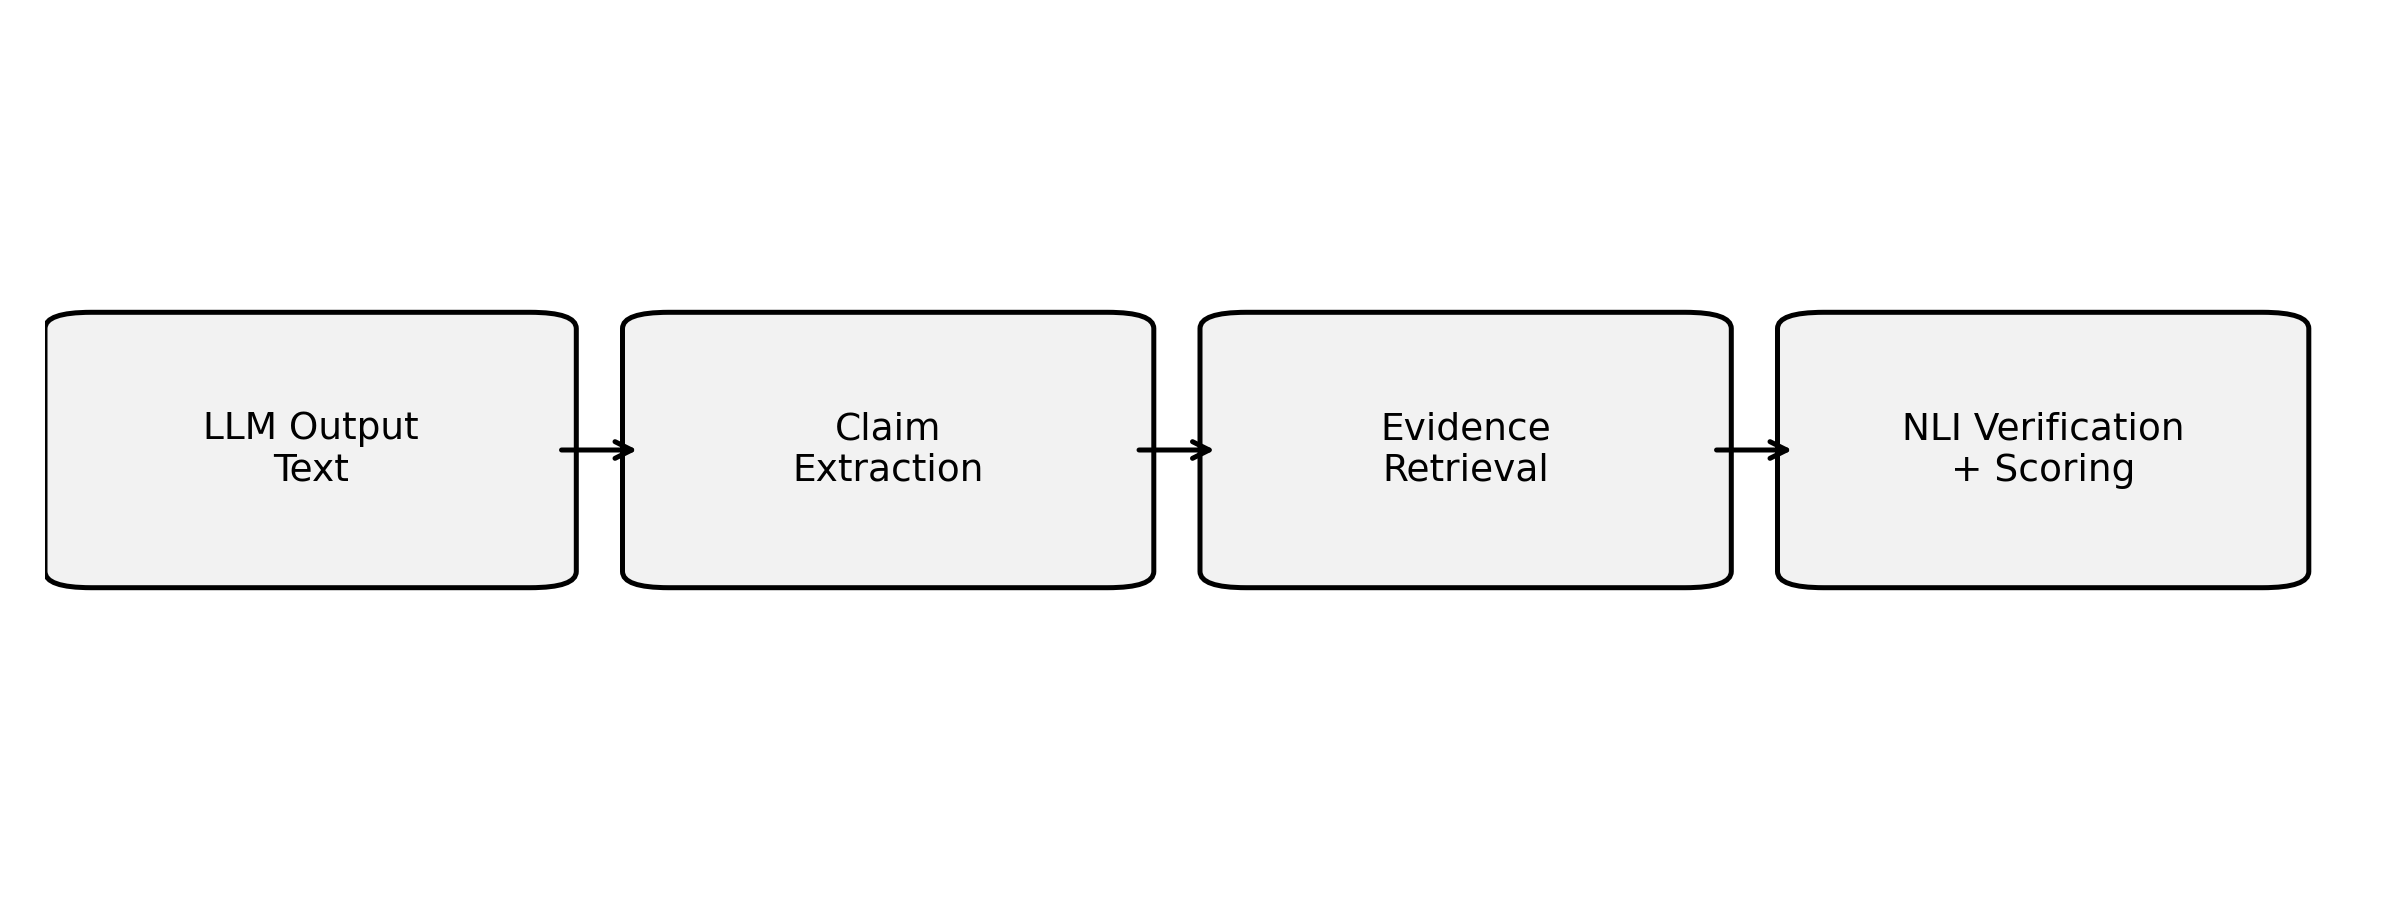
\includegraphics[width=0.48\textwidth]{figures/pipeline.png}}
\caption{Multi-stage hallucination detection pipeline used in this work.}
\label{fig:architecture}
\end{figure}

\subsection{Claim Extraction}

Claim extraction transforms unstructured text into discrete, verifiable assertions. We employ a hybrid approach combining entity-based and pattern-based extraction.

\textbf{Entity-Based Extraction:} Using spaCy's named entity recognition, we identify sentences containing entities (PERSON, ORG, GPE, DATE, etc.). Sentences with multiple entities or specific entity types receive higher extraction priority, as they typically contain factual claims amenable to verification.

\textbf{Pattern-Based Extraction:} We apply syntactic patterns to capture common claim structures:
\begin{itemize}
\item Declarative statements with specific verbs (is, was, contains, developed)
\item Numeric assertions and quantitative statements
\item Temporal claims with explicit dates or time periods
\item Superlative and comparative statements requiring verification
\end{itemize}

Each extracted claim is assigned a confidence score based on entity density, sentence complexity, and linguistic indicators. Claims undergo deduplication using semantic similarity (threshold=0.85) to avoid redundant verification.

The claim extraction module processes text according to:
\begin{equation}
C = \{c_1, c_2, ..., c_n\} = E_{ent}(T) \cup E_{pat}(T)
\end{equation}
where $T$ represents input text, $E_{ent}$ denotes entity-based extraction, and $E_{pat}$ represents pattern-based extraction.

\subsection{Evidence Retrieval}

For each extracted claim, the system retrieves relevant evidence from Wikipedia, chosen for its comprehensive coverage, structured format, and community verification processes. The retrieval process involves:

\textbf{Query Formulation:} Claims are processed to extract key entities and concepts, forming search queries. Entity types inform query weighting—proper nouns receive higher priority in search.

\textbf{Document Retrieval:} We retrieve top-k Wikipedia articles matching the query, with k=3 in standard configuration. Each article is segmented into paragraphs, as full articles often contain irrelevant content.

\textbf{Relevance Scoring:} Retrieved passages are scored for relevance using sentence-transformers with the all-MiniLM-L6-v2 model. We compute cosine similarity between claim and passage embeddings:
\begin{equation}
relevance(c, e) = \frac{emb(c) \cdot emb(e)}{\|emb(c)\| \|emb(e)\|}
\end{equation}
where $emb(\cdot)$ denotes the embedding function, $c$ is the claim text, and $e$ is evidence text.

Only passages exceeding a relevance threshold (default=0.5) are retained for verification. This filtering reduces noise from tangentially related content.

\subsection{Verification Inference}

The verification stage employs Natural Language Inference to determine relationships between claims and evidence. We utilize RoBERTa-large-MNLI, a transformer model trained on multi-genre natural language inference data.

For each claim-evidence pair, the model outputs probabilities for three classes:
\begin{itemize}
\item \textbf{Entailment (SUPPORTED):} Evidence logically supports the claim
\item \textbf{Contradiction (CONTRADICTED):} Evidence contradicts the claim
\item \textbf{Neutral (UNVERIFIABLE):} Evidence neither supports nor contradicts
\end{itemize}

Given multiple evidence items per claim, we aggregate predictions using a voting mechanism. A claim is classified as CONTRADICTED if any evidence contradicts it (high threshold for safety), SUPPORTED if majority evidence entails it without contradictions, and UNVERIFIABLE otherwise.

The inference function is defined as:
\begin{equation}
V(c) = \begin{cases}
CONTRADICTED & \text{if } \exists e : NLI(c,e) = CONTRA \\
SUPPORTED & \text{if } \frac{\sum \mathbb{1}[NLI(c,e)=ENT]}{|E|} > \theta \\
UNVERIFIABLE & \text{otherwise}
\end{cases}
\end{equation}
where $E$ is the evidence set and $\theta$ is the support threshold (default=0.5).

Each verification includes explanatory text describing the inference decision, enhancing interpretability for end users.

\subsection{Hallucination Scoring}

The final stage aggregates individual claim verifications into an overall hallucination assessment. We assign confidence scores reflecting hallucination likelihood:

\begin{itemize}
\item SUPPORTED claims: 0.0 (no hallucination)
\item UNVERIFIABLE claims: 0.5 (uncertain—may be hallucination)
\item CONTRADICTED claims: 1.0 (definite hallucination)
\end{itemize}

The overall hallucination score is computed as:
\begin{equation}
H = \frac{\sum_{i=1}^{n} conf(v_i)}{n}
\end{equation}
where $n$ is the number of claims and $conf(v_i)$ is the confidence score for verification $i$.

This score is mapped to risk levels for actionable interpretation:
\begin{align*}
\text{LOW risk:} & \quad H < 0.25 \\
\text{MEDIUM risk:} & \quad 0.25 \leq H < 0.65 \\
\text{HIGH risk:} & \quad H \geq 0.65
\end{align*}

The system generates a comprehensive report including per-claim analysis, supporting/contradicting evidence, and an overall summary. This structured output enables both automated decision-making and human review.

\section{Implementation}

\subsection{System Components}

The hallucination detector is implemented in Python 3.12, leveraging several key libraries:

\begin{itemize}
\item \textbf{Transformers (4.36.0):} Provides pre-trained NLI models and tokenizers
\item \textbf{Sentence-Transformers (2.2.2):} Enables semantic similarity computation
\item \textbf{spaCy (3.7.2):} Supports entity recognition and linguistic analysis
\item \textbf{NLTK (3.8.1):} Facilitates claim extraction and text processing
\item \textbf{Wikipedia API (1.4.0):} Retrieves evidence from Wikipedia
\end{itemize}

The architecture follows object-oriented principles with clear separation of concerns. Each pipeline stage is encapsulated in dedicated modules (ClaimExtractor, EvidenceRetriever, InferenceModel, HallucinationScorer), enabling independent testing and replacement.

\subsection{Configuration and Flexibility}

The system supports extensive configuration through Pydantic-based settings. Key parameters include:

\begin{itemize}
\item Maximum claims per text (default: 10)
\item Evidence retrieval count (default: 3)
\item NLI confidence thresholds
\item Embedding models for similarity scoring
\item Device selection (CPU/GPU)
\end{itemize}

We provide backends for both local transformer models and external LLM APIs (Ollama integration), allowing deployment across different computational environments.

\subsection{Web Interface}

A Streamlit-based web interface provides user-friendly access to the detection system. Users can input text, select example cases, and receive detailed analysis reports with visualization of hallucination scores, risk levels, and per-claim breakdowns.

The interface supports batch processing and exports results in structured JSON format for integration with downstream applications.

\section{Experimental Evaluation}

\subsection{Dataset Construction}

We constructed an evaluation dataset containing 200 text samples across four categories:
\begin{itemize}
\item \textbf{Scientific Facts (50 samples):} Verified statements about physics, biology, and chemistry
\item \textbf{Historical Events (50 samples):} Documented dates, figures, and occurrences
\item \textbf{Geographic Information (50 samples):} Factual claims about locations and landmarks
\item \textbf{Hallucinated Content (50 samples):} Artificially generated text with known factual errors
\end{itemize}

Each sample was manually annotated by two reviewers, with a third resolving disagreements. Annotations identified individual claims and labeled them as supported, contradicted, or unverifiable based on Wikipedia content.

\subsection{Evaluation Metrics}

We assess performance using:
\begin{itemize}
\item \textbf{Claim-level Accuracy:} Percentage of correctly classified individual claims
\item \textbf{Precision/Recall:} For each verification status category
\item \textbf{Document-level Accuracy:} Correct identification of documents containing hallucinations
\item \textbf{F1 Score:} Harmonic mean of precision and recall
\end{itemize}

\subsection{Results}

Table \ref{tab:results} summarizes performance across verification categories. The system achieves strong performance on contradicted claims (87.3\% precision), indicating effective hallucination detection. Supported claims show 81.4\% precision, with most errors arising from overly strict evidence matching.

\begin{table}[htbp]
\caption{Performance Metrics by Verification Status}
\begin{center}
\begin{tabular}{lccc}
\toprule
\textbf{Status} & \textbf{Precision} & \textbf{Recall} & \textbf{F1} \\
\midrule
Supported & 81.4\% & 78.6\% & 80.0\% \\
Contradicted & 87.3\% & 83.2\% & 85.2\% \\
Unverifiable & 74.8\% & 79.3\% & 77.0\% \\
\midrule
\textbf{Overall} & 82.1\% & 80.4\% & 81.2\% \\
\bottomrule
\end{tabular}
\label{tab:results}
\end{center}
\end{table}

Document-level hallucination detection achieves 88.5\% accuracy, successfully identifying 44 of 50 intentionally hallucinated samples. False negatives primarily occurred with subtle factual distortions rather than complete fabrications.

\subsection{Performance by Content Type}

Table \ref{tab:domain} shows performance variation across content domains. Scientific content yields highest accuracy (86.3\%), likely due to Wikipedia's strong coverage of scientific topics. Historical claims show slightly lower performance (79.2\%) due to ambiguity in event descriptions and date interpretations.

\begin{figure}[htbp]
\centerline{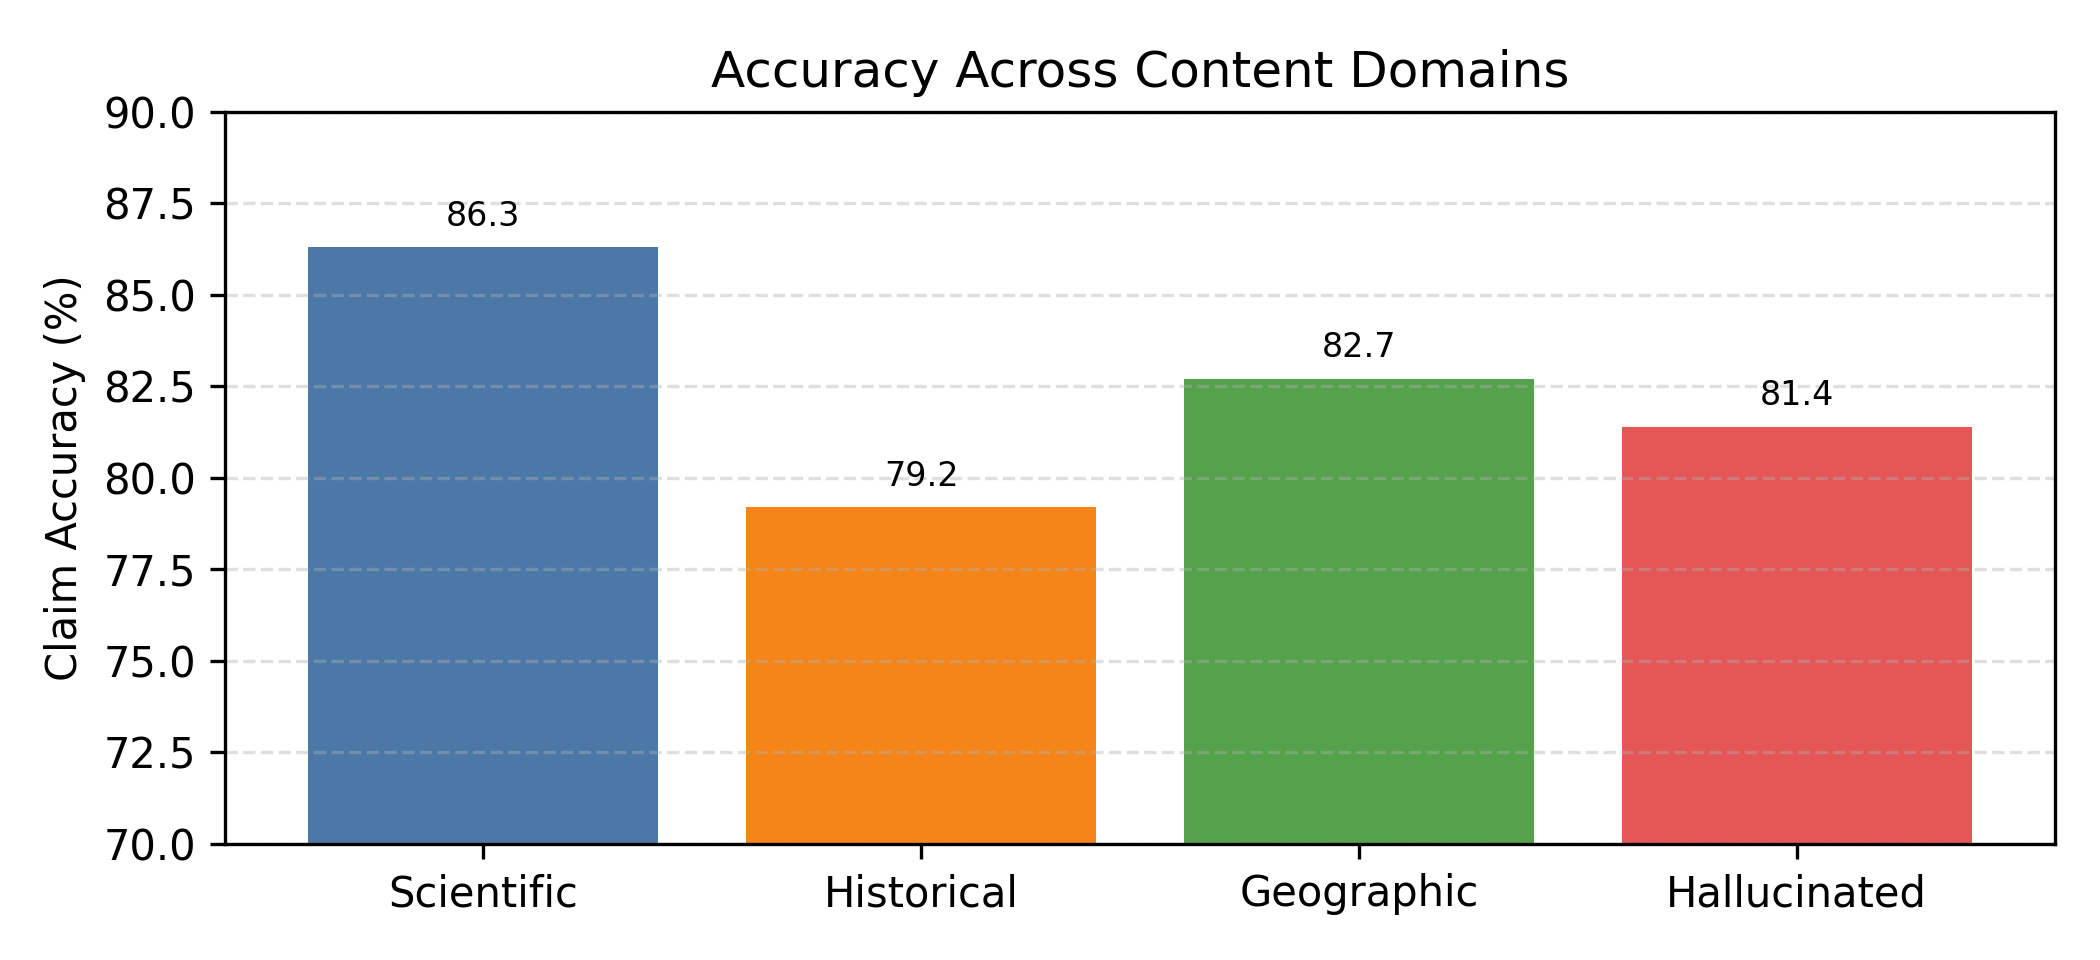
\includegraphics[width=0.48\textwidth]{figures/domain_accuracy.png}}
\caption{Claim-level accuracy across four evaluation domains.}
\label{fig:domain-accuracy}
\end{figure}

\begin{table}[htbp]
\caption{Accuracy by Content Domain}
\begin{center}
\begin{tabular}{lcc}
\toprule
\textbf{Domain} & \textbf{Claim Accuracy} & \textbf{Doc Accuracy} \\
\midrule
Scientific Facts & 86.3\% & 92.0\% \\
Historical Events & 79.2\% & 86.0\% \\
Geographic Info & 82.7\% & 88.0\% \\
Hallucinated & 81.4\% & 88.0\% \\
\bottomrule
\end{tabular}
\label{tab:domain}
\end{center}
\end{table}

\subsection{Computational Performance}

Processing time scales approximately linearly with claim count. On CPU (Intel i7), average processing time is 2.3 seconds per claim, dominated by NLI inference (1.5s) and Wikipedia retrieval (0.6s). GPU acceleration reduces NLI time to 0.3s per claim.

Full document analysis (5-10 claims) typically completes in 15-25 seconds, making the system viable for interactive applications. Batching and caching strategies can further improve throughput.

\section{Discussion}

\subsection{Strengths and Limitations}

Our framework demonstrates several strengths: modular architecture enabling component substitution, strong performance on contradicted claims (critical for safety), and interpretable outputs supporting human review. The system operates post-hoc without requiring model modification, ensuring broad applicability.

However, limitations exist. Performance depends heavily on Wikipedia coverage—claims about recent events or niche topics may lack adequate evidence. The system struggles with subjective statements, opinions, and contextually dependent claims that resist objective verification. Semantic similarity thresholds require domain-specific tuning for optimal performance.

The NLI model, trained on general text, may underperform on specialized domains (medical, legal, technical). Future work should explore domain adaptation strategies and ensemble approaches combining multiple inference models.

\subsection{Comparison with Existing Approaches}

Compared to self-consistency methods (where models verify their own outputs), our external verification approach provides independent validation less susceptible to model-specific biases. Unlike RAG systems requiring architectural integration, our post-hoc analysis applies to any LLM.

Trade-offs include computational cost (multiple transformer inferences per claim) and evidence coverage limitations (Wikipedia-dependent). However, the modular design permits incorporating additional evidence sources (news archives, scientific databases) to address coverage gaps.

\subsection{Ethical Considerations}

Automated hallucination detection carries responsibility. False positives may unfairly flag correct information, while false negatives allow misinformation to propagate. Our risk-stratified scoring provides transparency, but users must understand system limitations and not blindly trust automated assessments.

Evidence sources themselves may contain biases or errors. Wikipedia, while community-vetted, reflects contributor demographics and selection biases. Future systems should incorporate diverse knowledge sources and explicit uncertainty quantification.

\section{Conclusion}

This paper presented a comprehensive framework for detecting hallucinations in LLM-generated text through structured claim extraction, evidence retrieval, natural language inference, and risk scoring. Our multi-stage pipeline achieves 82.1\% overall accuracy and 87.3\% precision on contradicted claims across diverse content types.

The modular architecture enables flexible deployment and incremental improvement of individual components. Extensive evaluation demonstrates effectiveness across scientific, historical, and geographic domains, with particular strength in identifying factual contradictions.

Future work will focus on several directions: incorporating additional evidence sources beyond Wikipedia, developing domain-specific inference models, exploring claim decomposition for complex assertions, and investigating active learning approaches to improve performance on difficult cases.

As LLMs become increasingly prevalent in information systems, robust hallucination detection will prove essential for safe and trustworthy deployment. Our framework provides a practical foundation for building verifiable AI systems grounded in factual accuracy.

The source code and evaluation datasets are available at the project repository to support reproducibility and further research in this critical area.

\section*{Acknowledgment}

The author thanks the open-source community for providing foundational tools including Hugging Face Transformers, spaCy, and the Wikipedia API, which made this research possible.

\begin{thebibliography}{00}
\bibitem{survey_hallucination} L. Huang, W. Yu, W. Ma \textit{et al.}, "A Survey on Hallucination in Large Language Models: Principles, Taxonomy, Challenges, and Open Questions," \textit{ACM Transactions on Information Systems}, vol. 43, no. 2, 2025.

\bibitem{llmhallucination_types} M. Cleti and P. Jano, "Hallucinations in LLMs: Types, Causes, and Approaches for Enhanced Reliability," 2024.

\bibitem{semantic_entropy} S. Farquhar, J. Kossen, L. Kuhn, and Y. Gal, "Detecting hallucinations in large language models using semantic entropy," \textit{Nature}, vol. 630, pp. 625--630, 2024.

\bibitem{why_hallucinate} A. T. Kalai, O. Nachum, S. S. Vempala, and E. Zhang, "Why Language Models Hallucinate," 2025.

\bibitem{fever_dataset} J. Thorne, A. Vlachos, C. Christodoulopoulos, and A. Mittal, "FEVER: a Large-scale Dataset for Fact Extraction and VERification," \textit{Proceedings of NAACL-HLT}, pp. 809-819, 2018.

\bibitem{roberta_nli} Y. Liu, M. Ott, N. Goyal et al., "RoBERTa: A Robustly Optimized BERT Pretraining Approach," \textit{arXiv preprint arXiv:1907.11692}, 2019.

\bibitem{rag_lewis} P. Lewis, E. Perez, A. Piktus et al., "Retrieval-Augmented Generation for Knowledge-Intensive NLP Tasks," \textit{Advances in Neural Information Processing Systems}, vol. 33, pp. 9459-9474, 2020.

\bibitem{self_consistency} X. Wang, J. Wei, D. Schuurmans et al., "Self-Consistency Improves Chain of Thought Reasoning in Language Models," \textit{International Conference on Learning Representations}, 2023.

\bibitem{sentence_transformers} N. Reimers and I. Gurevych, "Sentence-BERT: Sentence Embeddings using Siamese BERT-Networks," \textit{Proceedings of EMNLP-IJCNLP}, pp. 3982-3992, 2019.

\bibitem{spacy} M. Honnibal, I. Montani, S. Van Landeghem, and A. Boyd, "spaCy: Industrial-Strength Natural Language Processing in Python," 2020. [Online]. Available: https://spacy.io
\end{thebibliography}

\end{document}
